\documentclass[12pt]{article}

\usepackage[english]{babel}
\usepackage[latin1]{inputenc}
\usepackage{amsmath}
\usepackage{enumitem}
\usepackage{graphicx}
\usepackage{ulem}
\usepackage{caption}
\usepackage{placeins}
\usepackage[usenames,dvipsnames]{color}
\usepackage[colorinlistoftodos]{todonotes}
\usepackage{listings}
\usepackage{fixltx2e}
\usepackage{scrpage2}
\usepackage{lastpage}
\clearscrheadfoot
\pagestyle{scrheadings}
\usepackage{glossaries}
\usepackage[
top    = 2.75cm,
bottom = 2.00cm,
left   = 2.50cm,
right  = 2.00cm]{geometry}
\setcounter{secnumdepth}{4}


\makeglossaries

\newglossaryentry{glossaryVerweis} {name=abkuerzung, description={Langer Name}}


\begin{document}
\begin{titlepage}
\begin{center}
% Oberer Teil der Titelseite:

\includegraphics[width=0.5\textwidth]{images/logo}\\[1cm]    

\textsc{\LARGE Technologisches Gewerbe Museum}\\[1.5cm]

% Title
\rule{12cm}{1mm}
{ \huge \bfseries  \\\large DezSys \\ \huge PI Calculator \\[0.4cm] }

\rule{12cm}{1mm}

% Author and supervisor
\noindent 
\vspace{5cm}

\begin{center}
\large
Author: 
P�cher \textsc{Ren�} \&
Steinkellner \textsc{Sebastian}
\end{center}

\vfill

% Bottom of the page
{\large \today}

\end{center}
\end{titlepage}

\tableofcontents


%HEADER AND FOOTER
\pagenumbering{arabic}
\ohead{\headmark}
\automark{section}
\ifoot{@Authors}
\ofoot{\pagemark ~of \pageref{LastPage}}

\newpage

\section{Aufgabe}

{\centering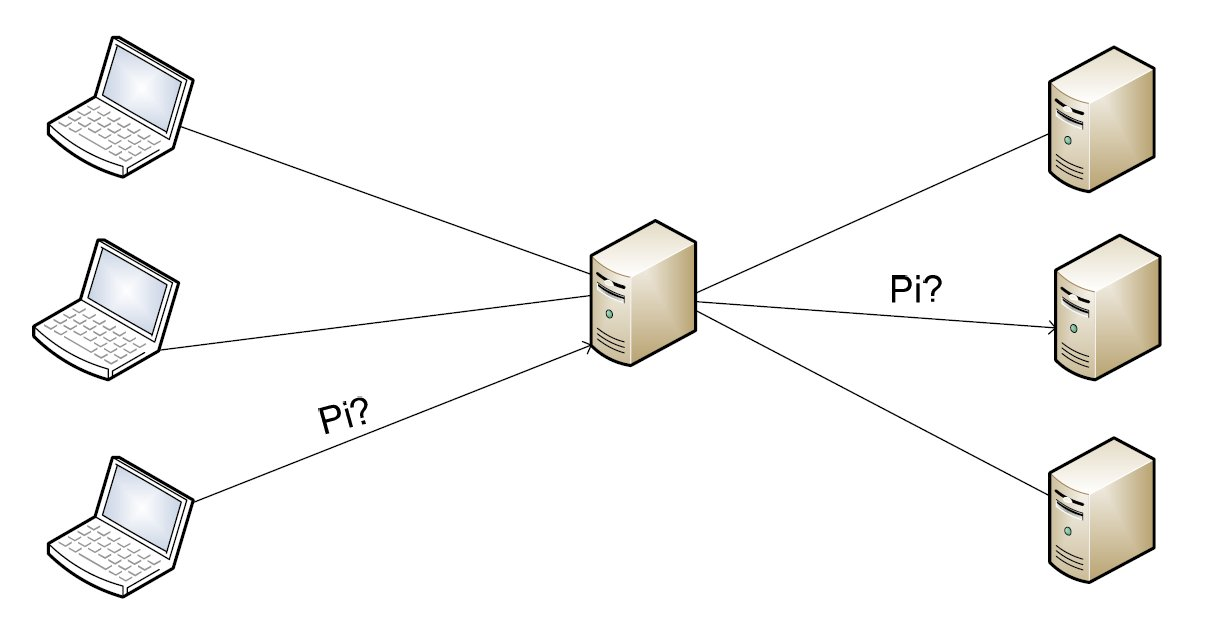
\includegraphics[width=10.5cm]{aufgabe1}}
\\
Als Dienst soll hier die beliebig genaue Bestimmung von pi betrachtet werden. Der Dienst stellt folgendes Interface bereit:
\\\\

// Calculator.java \\
public interface Calculator \{ \\
public BigDecimal pi (int anzahl\_nachkommastellen); \\
\}
\\\\\\
Ihre Aufgabe ist es nun, zun�chst mittels Java-RMI die direkte Kommunikation zwischen Klient und Dienst zu erm�glichen und in einem zweiten Schritt den Balancierer zu implementieren und zwischen Klient(en) und Dienst(e) zu schalten. Gehen Sie dazu folgendermassen vor:
\\\\	
Entwicklen Sie ein Serverprogramm, das eine CalculatorImpl-Instanz erzeugt und beim RMI-Namensdienst registriert. Entwicklen Sie ein Klientenprogramm, das eine Referenz auf das Calculator-Objekt beim Namensdienst erfragt und damit pi bestimmt. Testen Sie die neu entwickelten Komponenten.
\\\\
Implementieren Sie nun den Balancierer, indem Sie eine Klasse CalculatorBalancer von Calculator ableiten und die Methode pi() entsprechend implementieren. Dadurch verh�lt sich der Balancierer aus Sicht der Klienten genauso wie der Server, d.h. das Klientenprogramm muss nicht ver�ndert werden. Entwickeln Sie ein Balanciererprogramm, das eine CalculatorBalancer-Instanz erzeugt und unter dem vom Klienten erwarteten Namen beim Namensdienst registriert. Hier ein paar Details und Hinweise:
\\\\\\
Da mehrere Serverprogramme gleichzeitig gestartet werden, sollten Sie das Serverprogramm so erweitern, dass man beim Start auf der Kommandozeile den Namen angeben kann, unter dem das CalculatorImpl-Objekt beim Load-Balancer gespeichert wird. Damit soll der Server nun seine exportierte Instanz an den Balancer �bergeben, ohne es in die Registry zu schreiben. Verwenden Sie dabei ein eigenes Interface des Balancers, welches in die Registry gebinded wird, um den Servern das Anmelden zu erm�glichen.\\\\
Das Balancierer-Programm sollte nun den Namensdienst in festgelegten Abst�nden abfragen um herauszufinden, ob neue Server Implementierungen zur Verf�gung stehen.
Java-RMI verwendet intern mehrere Threads, um gleichzeitig eintreffende Methodenaufrufe parallel abarbeiten zu k�nnen. Das ist einerseits von Vorteil, da der Balancierer dadurch mehrere eintreffende Aufrufe parallel bearbeiten kann, andererseits m�ssen dadurch im Balancierer �nderbare Objekte durch Verwendung von synchronized vor dem gleichzeitigen Zugriff in mehreren Threads gesch�tzt werden.\\\\
Beachten Sie, dass nach dem Starten eines Servers eine gewisse Zeit vergeht, bis der Server das CalculatorImpl-Objekt erzeugt und beim Namensdienst registriert hat sich beim Balancer meldet. D.h. Sie m�ssen im Balancierer zwischen Start eines Servers und Abfragen des Namensdienstes einige Sekunden warten.


\newpage

\section{Working time}
\subsection{Estimated Working time}
\begin{center}
\textbf{Estimated working time}
\end{center}

\begin{table}[h]

\begin{tabular}{|p{0.4\textwidth}|p{0.2\textwidth}|p{0.2\textwidth}|}
\hline
\textbf{Task}    & \textbf{Person}                                               & \textbf{Time in hours                              } \\ \hline \hline
Planung  & \begin{tabular}[c]{c}P�cher\\ Steinkellner\end{tabular} & \begin{tabular}[c]{c}1\end{tabular}    \\ \hline 
UML Design & \begin{tabular}[c]{c}P�cher\end{tabular} & \begin{tabular}[c]{c}1/2\end{tabular}    \\ \hline 
PI Methode desig. \& Implementieren  & \begin{tabular}[c]{c}P�cher\end{tabular} & \begin{tabular}[c]{c}2\end{tabular}    \\ \hline \hline
Total & \begin{tabular}[c]{c}P�cher\\ Steinkellner\end{tabular} & \begin{tabular}[c]{c}2 1/2\\1\end{tabular}   \\ \hline 
\textbf{Total Team} & & \textbf{4 hours}  \\ \hline 
\end{tabular}
\caption{Estimated working time}
\end{table}


\newpage

\section{Easy Bibliography}
\listoftables
\listoffigures
\printglossaries

\begin{thebibliography}{56}

\bibitem{name}
   \textbf{Who}, When\\
  \textit{url}
  \newline last used: dd.mm.yyyy, hh:mm
 
 \bibitem{example} 
  \textbf{Mister Super-genious}, Answer from 20.01.2015\\
  \textit{http://www.stackoverflow.com/question}
  \newline last used: 22.10.2014, 21:00
\end{thebibliography}
\end{document}
